\documentclass{report}

\input{preamble}

\input{macros}
\input{letterfonts}
\usepackage{verbatim} % comentarios
\usepackage{amsmath} % teoremas
\usepackage{amsthm} % teoremas
\usepackage{amssymb} % teoremas


\title{\Huge{Estadísticas y probabilidades}\\2023-1}
\author{\huge{Lenin Chavez}}
\date{}

\begin{document}

\maketitle
\newpage% or \cleardoublepage
% \pdfbookmark[<level>]{<title>}{<dest>}
\pdfbookmark[section]{\contentsname}{toc}
\tableofcontents
\pagebreak

\chapter{}
\section{Muestreo aleatorizado}
\dfn{}{\textbf{MUESTREO ALEATORIO :} es aquel procedimiento de selección de la muestra en el que todos y cada uno de los elementos de la población tiene una cierta probabilidad de resultar elegidos. (uv.es)}

\dfn{}{\textbf{MUESTREO ALEATORIO SIMPLE :} Elegir una muestra representativa de la población en la que cada elemento de la población tiene la misma probabilidad de ser elegido y todas las muestras del mismo tamaño son igualmente probables.} \nt{Cuidado con los "unicornios"}
\dfn{}{\textbf{MUESTREO ALEATORIO ESTRATIFICADO :} es aquel en el que la población se divide en subpoblaciones o estratos y se elige una muestra aleatoria simple de cada estrato, de manera que en nuestra muestra total la relación entre la población de los estratos y sus unidades muestrales sea de manera proporcinal.}
\nt{Garantiza representatividad de los estratos. Por ejemplo, si un estrato representa el 1/6 de la población, entonces 1/6 de nuestra muestra debe ser de ese estrato.}
\dfn{}{\textbf{MUESTREO ALEATORIO POR CONGLOMERADOS :}  Asume que todos los conglomerados son equivalentes y que cada uno de ellos tiene la misma probabilidad de ser elegido.}

\subsection{Debilidades del muestreo aleatorizado}
\begin{itemize}
	\item M.A.S
	      \begin{itemize}
		      \item Es necesario tener acceso explícito a toda la población
		      \item Es potencialmente costoso y demandante de tiempo
	      \end{itemize}
	\item M.E.
	      \begin{itemize}
		      \item El conocimiento sobre los estratos y sus tamaños es imorescindible
		      \item Es necesario acceso a todos los estratos y sus U.M.
	      \end{itemize}
	\item M.C.
	      \begin{itemize}
		      \item Es necesario que los conglomerados sean genuinamente parecidos
		      \item Hay conglomerados que no se muestrean
	      \end{itemize}
\end{itemize}
\nt{El resultado típico de tomar una muestra es una tabla de datos.}
\section{Tabla de datos}
\dfnc{}{\textbf{Tabla de datos :} es prolija si tiene una observación por fila y una variable por columna.}
\begin{comment}
\clm{Topology}{}{Topology is cool}
\ex{Open Set and Close Set}{
	\begin{tabular}{rl}
		Open Set:   & $\bullet$ $\phi$                                              \\
		            & $\bullet$ $\bigcup\limits_{x\in X}B_r(x)$ (Any $r>0$ will do) \\[3mm]
		            & $\bullet$ $B_r(x)$ is open                                    \\
		Closed Set: & $\bullet$ $X,\ \phi$                                          \\
		            & $\bullet$ $\overline{B_r(x)}$                                 \\
		            & $x-$axis $\cup$ $y-$axis
	\end{tabular}}
\thm{}{If $x\in$ open set $V$ then $\exists$ $\delta>0$ such that $B_{\delta}(x)\subset V$}
\begin{myproof}By openness of $V$, $x\in B_r(u)\subset V$
	\begin{center}
		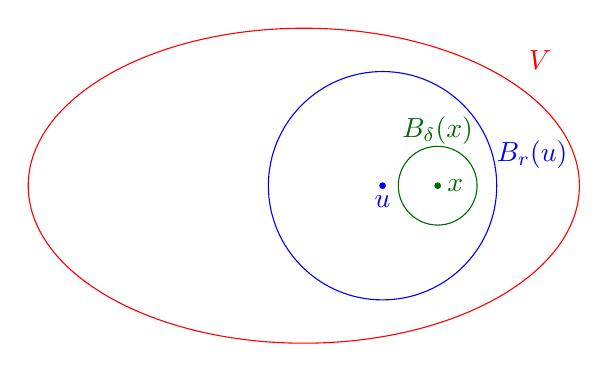
\begin{tikzpicture}
			\draw[red] (0,0) circle [x radius=3.5cm, y radius=2cm] ;
			\draw (3,1.6) node[red]{$V$};
			\draw [blue] (1,0) circle (1.45cm) ;
			\filldraw[blue] (1,0) circle (1pt) node[anchor=north]{$u$};
			\draw (2.9,0.4) node[blue]{$B_r(u)$};
			\draw [green!40!black] (1.7,0) circle (0.5cm) node [yshift=0.7cm]{$B_{\delta}(x)$} ;
			\filldraw[green!40!black] (1.7,0) circle (1pt) node[anchor=west]{$x$};
		\end{tikzpicture}
	\end{center}

	Given $x\in B_r(u)\subset V$, we want $\delta>0$ such that $x\in B_{\delta} (x)\subset B_r(u)\subset V$. Let $d=d(u,x)$. Choose $\delta $ such that $d+\delta<r$ (e.g. $\delta<\frac{r-d}{2}$)

	If $y\in B_{\delta}(x)$ we will be done by showing that $d(u,y)<r$ but $$d(u,y)\leq d(u,x)+d(x,y)<d+\delta<r$$
\end{myproof}

\cor{}{By the result of the proof, we can then show...}
\mlenma{}{Suppose $\vec{v_1}, \dots, \vec{v_n} \in \RR[n]$ is subspace of $\RR^n$.}
\mprop{}{$1 + 1 = 2$.}


\end{comment}




\section{Tipos de variables}
\dfnc{}{\textbf{Variable :} es una característica que puede tomar diferentes valores.}
\begin{itemize}
	\item {\textbf{Variable numérica :} es una variable que puede tomar valores numéricos.} \begin{itemize}
		      \item {\textbf{Variable discreta :} es una variable que puede tomar valores numéricos enteros. Se puede contar, ordenar, aritmética.}
		      \item {\textbf{Variable continua :} es una variable que puede tomar valores numéricos reales. Se puede contar, ordenar, aritmética.}
	      \end{itemize}
	\item {\textbf{Variable categórica :} es una variable que puede tomar valores no numéricos.} \begin{itemize}
		      \item {\textbf{Variable nominal :} es una variable que puede tomar valores no numéricos que no tienen orden. Se puede contar.}
		      \item {\textbf{Variable ordinal :} es una variable que puede tomar valores no numéricos que tienen orden.Se puede contar, ordenar.}
	      \end{itemize}

\end{itemize}
\begin{comment}
\begin{algorithm}[H]
	\KwIn{This is some input}
	\KwOut{This is some output}
	\SetAlgoLined
	\SetNoFillComment
	\tcc{This is a comment}
	\vspace{3mm}
	some code here\;
	$x \leftarrow 0$\;
	$y \leftarrow 0$\;
	\uIf{$ x > 5$} {
		x is greater than 5 \tcp*{This is also a comment}
	}
	\Else {
		x is less than or equal to 5\;
	}
	\ForEach{y in 0..5} {
		$y \leftarrow y + 1$\;
	}
	\For{$y$ in $0..5$} {
		$y \leftarrow y - 1$\;
	}
	\While{$x > 5$} {
		$x \leftarrow x - 1$\;
	}
	\Return Return something here\;
	\caption{what}
\end{algorithm}
\end{comment}
\section{Limpieza de datos}
\begin{itemize}
	\item {\textbf{Política de subsanación de errores}: Puedes eliminar todo lo que tenga errores, intentar arreglar el error(si haces esto la mejor opción es preguntar a la fuente original ya que de lo contrario estarías suponiendo y puede contaminar la muestra, reemplazarlos por N.A)}
	\item {\textbf{Política de manejo de errores :}Eliminar todo lo que tiene datos faltantes, intentar llenar los datos faltantes(Mejor opción es preguntar a la fuente original, la otra opción es técnicas de imputación), vivir con ellos lo cuál es peligroso para la muestra}
\end{itemize}
\section{Descriptores}
\begin{itemize}

	\item {\textbf{Numéricos}:}
	      - Es un número que trata de resumir algo sobre los datos: Hay de posición(Moda, mediana, promedio), dispersión(rango, rango intercuartil, varianza, desviación estándar) e interacción(covarianza, correlación).
	\item {\textbf{Gráficos}:}
	      - Un conjunto de números junto con una visualización tratan de resumir algo sobre los datos hay de posición(diagramas de barras, puntos, lineas, histogramas), dispersión(caja y bigotes) e interacción(diagramas disp., boxplots indexados, mosaicos) .
	      \item{\textbf{Tabulares}:}
	      - Listas de valores extaídos de la muestra( típicamente, tablas de frecuencia)


\end{itemize}

\chapter{}

\section{Experimento aleatorio}

$\Omega F P$ Modelo de un expermiento aleatorio.\\
$\Omega$: Espacio de todos los resultados de posibles interés.\\
$F \subseteq 2^\Omega \rightarrow$ F: Álgebra de eventos, $2^\Omega$: conjunto de partes de $\Omega$\\
$F$: Están todos los eventos de interés. $F$ es un conjunto de conjuntos que debe cumplir condiciones técnicas. Las uniones, intersecciones, complementos, etc de eventos son eventos.\\
$P$ es una función de conjuntos que a cada conjunto en $F$ le asigna un número entre 0 y 1 conocido como su probabilidad. $P$ tambien debe cumpli condiciones técnicas.\\

\[
	P = F \rightarrow [0,1]
\]




Las condiciones técnicas deben obedecer los siguientes axiomas.

\begin{align*}
	\text{Axioma 1: }\forall A \in F, P(A) \geq 0  \\
	\text{Axioma 2: }P(\Omega) = 1                 \\
	\text{Axioma 3: }\forall A_1, A_2, \dots \in F \\ \text{ disjuntos } P(\bigcup_{i=1}^{\infty} A_i) = \sum_{i=1}^{\infty} P(A_i) \\
\end{align*}

Propiedades de P: \\

\begin{itemize}
	\item	\text{Propiedad 1: }$P(\emptyset) = 0  $
	\item	\text{Propiedad 2: }$P(\bar{A}) = 1 - P(A)  $
	\item	\text{Propiedad 3: } Si A, B $\in$ F y A $\cap$ B = $\emptyset$ entonces, $P(A \cup B) = P(A) + P(B) $
	\item	\text{Propiedad 4: } Si A, B $\in$ F entonces $P(A \cup B) = P(A) + P(B) - P(A \cap B) $
	\item	\text{Propiedad 5: } Si A, B $\in$ F y A $\subseteq$ B entonces $P(A) \leq P(B) $
\end{itemize}

\nt{ La $P$ nos da una forma alterna de "medir" el tamaño de un conjunto}

\ex{Lanzamiento de una moneda justa}{
	$\Omega_1$ = \{cara, sello\} \\
	$F_1$ = \{ $\emptyset$, \{cara\}, \{sello\}, \{cara, sello\} \} \\
	$P_1$ = \{ $\emptyset$ = 0, \{cara\} = 1/2, \{sello\} = 1/2, \{cara, sello\} = 1 \} \\

}

\ex{Lanzamos un dado de seis caras, juusto y anotamos el resultado}{
	$\Omega_2$ = \{1,2,3,4,5,6\} \\
	$F_2$ = \{$\emptyset$,
	\{1\}, \{2\}, \{3\}, \{4\}, \{5\}, \{6\},
	\{1,2\}, \{1,3\}, \{1,4\}, \{1,5\}, \{1,6\},
	\{2,3\}, \{2,4\}, \{2,5\}, \{2,6\}, \dotso \} \\
	$P_2(\text{sale par})$ = 1/2 \\
	$P_2(\text{sale impar})$ = 1/2 \\
	$P_2(\text{sale 1})$ = 1/6 \\
	$P_2(\text{no sale 1})$ = 5/6 \\
}

\ex{Lanzo un dado justo y anoto que sale pero si sale 4, 5 o 6 anoto No en vez}{
	$\Omega_3$ = \{1,2,3,No\} \\
	$F_3$ = $2^{\Omega_3}$ \\
	$|F_3|$ = 16 \\
	Usando EA del siguiente ejemplo \\
	$P_3$(\{i\}) = 1/6 \\
	$P_3$(Sale 3 o No) = 4/6 \\
}

\ex{Experimento accesorio
}
{

	Lanzo un dado justo y anoto lo que sale.\\
	$P_A$(\{4,5,6\}) = 1/2 \\
	$P_3$(\{1,2,3\}) = 1/2 \\
	$P_3$(\{No\}) = 1/2 \\
}
\dfn{EA: Experimento aleatorio}{
	($\Omega F P$)(Con $\Omega$ finito) Es un espacio \textbf{Equiprobable} si todos sus eventos atómicos tienen la misma probabilidad. E1, E2, EA son espacios Equiprobable, E3 no lo es.
	\\
	Cuando un espacio es equiprobable es fácil calcular probabilidades ($\Omega F P$) es equiprobable entonces:
	\[
		\forall x \in \Omega, P(\{x\}) = c
	\]
	\[
		P(A) = \sum_{x \in A} P(\{x\}) = \sum_{x \in A} c = c|A| = \frac{|A|}{|\Omega|}
	\]
	A es casos favorables y $\Omega$ es casos totales.

	ESTO SOLO FUNCIONA EN ESPACIOS EQUIPROBABLES.
}

\ex{Tenemos una bolsa con 6 bolas numeradas del 1 al 6 sacamos 3 bllas a la vez y anotamos lo que salió}{

	$\Omega_4$ = \{(x,y,z) / x,y,z $\in$ \{1,2,3,4,5,6\} \} \\
	$F_4$ = $2^{\Omega_4}$ \\
	$P_4$(\{(x,y,z) / x,y,z $\in$ \{1,2,3,4,5,6\} \}) = 1/20 \\
	$P_4$(\{(x,y,z) / x,y,z $\in$ \{1,2,3,4,5,6\} y x,y,z son distintos\}) = 6/20 \\
	$P_4$(\{(x,y,z) / x,y,z $\in$ \{1,2,3,4,5,6\} y x,y,z son iguales\}) = 1/20 \\

}


\end{document}
